\documentclass[11pt, a4paper, twocolumn]{article}
\font\myfont=cmr12 at 21pt
\title{{\myfont Jensen's Inequality}}
\date{31-07-2019}
\author{Claudiu Rediu}
\usepackage[utf8]{inputenc}
\usepackage[english]{babel}
\usepackage{amsthm}
\usepackage{amssymb}
\usepackage{amsmath}
\usepackage{graphicx}
\renewcommand\qedsymbol{$\blacksquare$}
\usepackage{float}
\theoremstyle{definition}
\newtheorem{definition}{Definition}

\begin{document}
	\pagenumbering{gobble}
	\maketitle
	\newpage
	\pagenumbering{arabic}
	\newpage
	
	\section*{Jensen's inequality}
		
	In mathematics, Jensen's inequality, named after the Danish mathematician Johan Jensen, relates the value of a convex function of an integral to the integral of the convex function. It was proven by Jensen in 1906. Given its generality, the inequality appears in many forms depending on the context, some of which are presented below. In its simplest form the inequality states that the convex transformation of a mean is less than or equal to the mean applied after convex transformation; it is a simple corollary that the opposite is true of concave transformations.
	
	Jensen's inequality generalizes the statement that the secant line of a convex function lies above the graph of the function, which is Jensen's inequality for two points: the secant line consists of weighted means of the convex function (for t $\in$ [0,1]).
	\begin{equation}
		f(tx_1 + (1-t)x_2) \leq tf(x_1) + (1-t)f(x_2)
	\end{equation}
	
	\begin{figure}[H]
	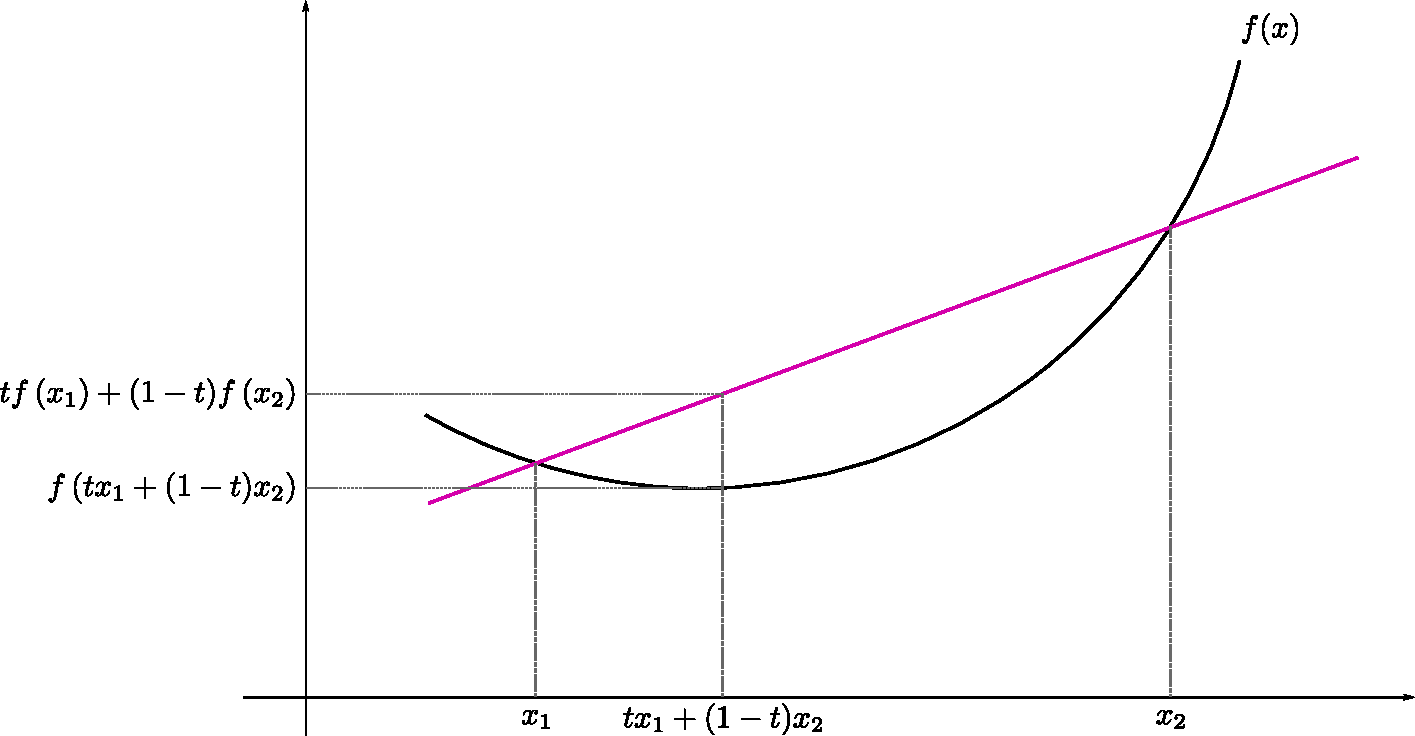
\includegraphics[width=\linewidth, height=120px]{ConvexFunction.pdf}
	\caption{A secant line of a convex function}
	\end{figure}

	In the context of Probability Theory it is used usually in this way:
	\begin{equation}
	f(\sum_{i=1}^{n}p_ix_i) \leq \sum_{i=1}^{n}p_if(x_i)
	\end{equation}
	
	\begin{proof}
		Let's show that f is convex on an interval if and only if for all $x_1$ and $x_2$ in the interval we have
		$$f(tx_1 + (1-t)x_2) \leq tf(x_1) + (1-t)f(x_2), \ \  0 < t < 1$$
		
		$$\frac{f(tx_1 + (1-t)x_2}{tx_1 + (1-t)x_2} \leq \frac{f(x_2) - f(x_1)}{x_2 - x_1}$$
		After working the inequality a bit, we end up with Jensen's Inequality
		$$f(tx_1 + (1-t)x_2) \leq tf(x_1) + (1-t)f(x_2)$$
		We're going to need a different approach to obtain Jensen's Inequality that is used mostly in Probability Theory. We will start with $\sum_{i=1}^{n}p_i = 1 $ for $n > 1$. We're going to show that for any numbers $x_1,...,x_n$ the sum $\sum_{i=1}^{n}p_ix_i$ is between the smallest and largest $x_i$
		
		We pick $x_\alpha$ to be the smallest one and $x_\beta$ to be the largest value. Then we end up with the inequality:
		$$\sum_{i=1}^{n}p_ix_\alpha < \sum_{i=1}^{n}p_ix_i < \sum_{i=1}^{n}p_ix_\beta$$
		$\sum_{i=1}^{n}p_ix_\alpha$ is equal to $x_\alpha$ and $\sum_{i=1}^{n}p_ix_\beta$ to $x_\beta$. Then this is done.
		
		The next step is to show the same for $\frac{1}{t}\sum_{i=1}^{n}p_ix_i$ where $t = \sum_{i=1}^{n-1}p_i$.
		
		What we've just shown applied to $\frac{p_1}{t},...,\frac{p_n}{t}$ shows that $\frac{1}{t}\sum_{i=1}^{n}p_ix_\alpha$ lies between the smallest and the largest $x_1,...,x_{n-1}$, so it certainly lies between $x_1,...,x_n$.
	
		We now can prove Jensen's Inequality in the context of Probability Theory
		\begin{equation*}
		\begin{split}
			f(\sum_{i=1}^{n}p_ix_i) &= f(t* \frac{1}{t}\sum_{i=1}^{n}p_ix_i +(1-t)x_n) \\
			& \leq tf(\sum_{i=1}^{n-1}\frac{p_i}{t}x_i) + (1-t)f(x_n) \\
			& \leq t\sum_{i=1}^{n-1}\frac{p_i}{t}f(x_i) + p_nf(x_n) \\
			& = \sum_{i=1}^{n}p_if(x_i)
		\end{split}
		\end{equation*}
		We end our proof with $f(\sum_{i=1}^{n}p_ix_i) \leq \sum_{i=1}^{n}p_if(x_i)$
	\end{proof}

\end{document}